\documentclass[11pt,]{article}
\usepackage{lmodern}
\usepackage{amssymb,amsmath}
\usepackage{ifxetex,ifluatex}
\usepackage{fixltx2e} % provides \textsubscript
\ifnum 0\ifxetex 1\fi\ifluatex 1\fi=0 % if pdftex
  \usepackage[T1]{fontenc}
  \usepackage[utf8]{inputenc}
\else % if luatex or xelatex
  \ifxetex
    \usepackage{mathspec}
  \else
    \usepackage{fontspec}
  \fi
  \defaultfontfeatures{Ligatures=TeX,Scale=MatchLowercase}
\fi
% use upquote if available, for straight quotes in verbatim environments
\IfFileExists{upquote.sty}{\usepackage{upquote}}{}
% use microtype if available
\IfFileExists{microtype.sty}{%
\usepackage{microtype}
\UseMicrotypeSet[protrusion]{basicmath} % disable protrusion for tt fonts
}{}
\usepackage[margin=1in]{geometry}
\usepackage{hyperref}
\PassOptionsToPackage{usenames,dvipsnames}{color} % color is loaded by hyperref
\hypersetup{unicode=true,
            pdftitle={On Pure Exploration, Thresholding Bandits, and Kullback-Leibler Divergence},
            colorlinks=true,
            linkcolor=Maroon,
            citecolor=Blue,
            urlcolor=blue,
            breaklinks=true}
\urlstyle{same}  % don't use monospace font for urls
\usepackage{longtable,booktabs}
\usepackage{graphicx,grffile}
\makeatletter
\def\maxwidth{\ifdim\Gin@nat@width>\linewidth\linewidth\else\Gin@nat@width\fi}
\def\maxheight{\ifdim\Gin@nat@height>\textheight\textheight\else\Gin@nat@height\fi}
\makeatother
% Scale images if necessary, so that they will not overflow the page
% margins by default, and it is still possible to overwrite the defaults
% using explicit options in \includegraphics[width, height, ...]{}
\setkeys{Gin}{width=\maxwidth,height=\maxheight,keepaspectratio}
\IfFileExists{parskip.sty}{%
\usepackage{parskip}
}{% else
\setlength{\parindent}{0pt}
\setlength{\parskip}{6pt plus 2pt minus 1pt}
}
\setlength{\emergencystretch}{3em}  % prevent overfull lines
\providecommand{\tightlist}{%
  \setlength{\itemsep}{0pt}\setlength{\parskip}{0pt}}
\setcounter{secnumdepth}{5}
% Redefines (sub)paragraphs to behave more like sections
\ifx\paragraph\undefined\else
\let\oldparagraph\paragraph
\renewcommand{\paragraph}[1]{\oldparagraph{#1}\mbox{}}
\fi
\ifx\subparagraph\undefined\else
\let\oldsubparagraph\subparagraph
\renewcommand{\subparagraph}[1]{\oldsubparagraph{#1}\mbox{}}
\fi

%%% Use protect on footnotes to avoid problems with footnotes in titles
\let\rmarkdownfootnote\footnote%
\def\footnote{\protect\rmarkdownfootnote}

%%% Change title format to be more compact
\usepackage{titling}

% Create subtitle command for use in maketitle
\newcommand{\subtitle}[1]{
  \posttitle{
    \begin{center}\large#1\end{center}
    }
}

\setlength{\droptitle}{-2em}
  \title{On Pure Exploration, Thresholding Bandits, and Kullback-Leibler
Divergence}
  \pretitle{\vspace{\droptitle}\centering\huge}
  \posttitle{\par}
  \author{}
  \preauthor{}\postauthor{}
  \date{}
  \predate{}\postdate{}

\usepackage[retainorgcmds]{IEEEtrantools}
\usepackage{bm}
\usepackage{amsmath}
\usepackage{bbm}
\usepackage{hyperref}
\usepackage[lined,boxed]{algorithm2e}
\newtheorem{theorem}{Theorem}
\newtheorem{definition}{Definition}
\newtheorem{lemma}{Lemma}
\newtheorem{corollary}{Corollary}
\newcommand{\KL}{\,\text{KL}}
\newcommand{\der}{\,\text{d}}
\newcommand*{\Alignyesnumber}{\refstepcounter{equation}\tag{\theequation}}%

\begin{document}
\maketitle

{
\hypersetup{linkcolor=black}
\setcounter{tocdepth}{2}
\tableofcontents
}
\newpage

\section{\texorpdfstring{Experiments
\label{chap:Experiments}}{Experiments }}\label{experiments}

We now compare the algorithms introduced in the previous chapters in
simulations and experiments against each other to evaluate their
performance. We first perform experiments on synthetic data in
\autoref{sec:SyntheticData}. We then use Bernoulli time series data
collected by the online shop Amorelie to evaluate the algorithms on real
world data in \autoref{sec:RealData}.

We compare the empirical performance of the SLR algorithm not only
against the APT algorithm, but also against the variance-based
algorithms. Thus we also compare the variance-based algorithms for the
first time directly against each other. As benchmark, the uniform
sampling strategy is included. Additionally, we include the Bayes-UCB
algorithm introduced in Kaufmann et al. (2012) for the cumulative regret
setting. See \autoref{sec:AppendixBUCB} in the appendix for how we adapt
the Bayes-UCB algorithm to the thresholding bandit problem.

\subsection{\texorpdfstring{Experiments on Web Analytics Data
\label{sec:RealData}}{Experiments on Web Analytics Data }}\label{experiments-on-web-analytics-data}

In the following, we present the results of two experiments performed on
a real world data set. While most multi-armed bandit algorithms are
assessed on synthetic data, as we have done in
\autoref{sec:SyntheticData}, a real world data set is useful to observe
how algorithms perform in presence of, for example, not perfectly i.i.d.
samples. Every experimenter of course tries to run their algorithms
under settings as ideal as possible, but there will always be problems.
Thus our experiments serve as a first robustness check on the algorithms
introduced before.

\subsubsection{The Data Set}\label{the-data-set}

Data have been collected by the German online shop
\href{https://amorelie.de}{Amorelie} as part of standard website
analytics. For 197 selected products, we observe the number of users
visiting each product's detail page (PDP) during a given minute. The
data set we use here has been collected during the entire month of
November 2016. It can be considered time series data sampled at minutely
frequency. Thus the data contain 43200 observations per product, and in
total 8510400 observations.

Since we would like to run an offline comparison of bandit algorithms,
it is important to have at each time point an observation for each arm.
Given that, it is easy to evaluate the perfomance of algorithms that
make different decisions at different point in times and thus do not
observe the same samples. By having an observation for each arm at any
given time point, each algorithm had at least the opportunity to observe
a certain sample. Other papers (for example, Li et al., 2011) have
solved this problem by using a sample drawn uniformly during, for
example, an A/B test. Then, if the next observation in the sample is not
from the same arm that the algorithm would like to draw from,
observations are discarded until the next observation from the selected
arm.

The choice of using what is essentially multivariate time series data as
the sample offers a simple way of running the algorithms just as often
on the real data as on simulated data. The goal is to perform 5000 runs
over the sample to confidently assess the performance. Since we would
like to preserve potential time dependencies in the data, a simple
resampling of the data is not an option to create the needed 5000
variations of the sample. Instead we perform time series cross
validation. To preserve the autocorrelation, one can create different
samples of \(n\) observations by sliding a window of size \(n\) over the
time series. Moving the window one period (in our case one minute) at a
time, one ensures that no sample shares start and end observation with
another sample (see Figure 8)\footnote{The graphic is adapted from a
  graphic by Rob J. Hyndman available at
  \url{https://gist.github.com/robjhyndman/9fa152c585442bb076eb42a30a020091}}.
In particular, this means for a given bandit strategy and two samples
that the observations that the algorithm collects as feedback during the
initialization phases differ from sample to sample and are never the
same. This is because during initialization every strategy pulls arms
\(1, ..., K\) (or \(1,...,2K\) for EVT) once in this order.

\begin{figure}

{\centering 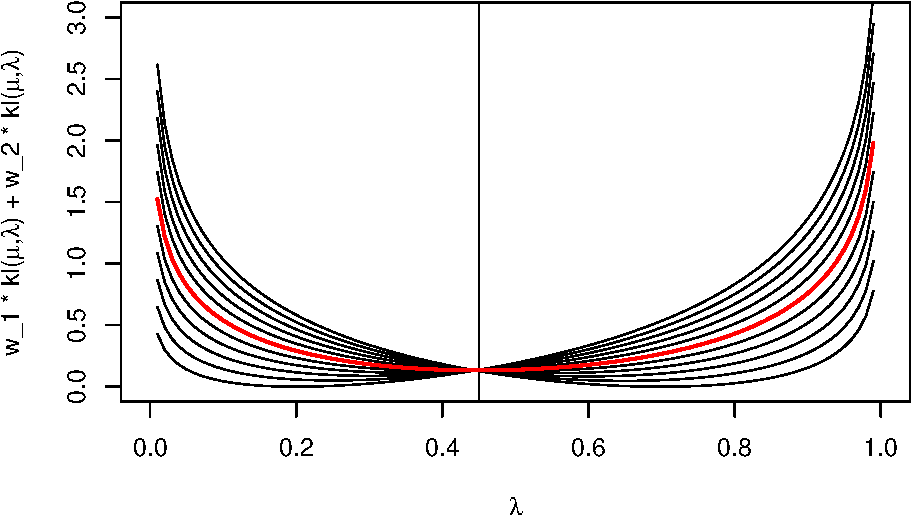
\includegraphics[width=0.8\linewidth]{Draft_for_Markus_files/figure-latex/unnamed-chunk-1-1} 

}

\caption{We use time series crossvalidation, to create many samples from one data set.}\label{fig:unnamed-chunk-1}
\end{figure}

While the data set consists of count data (the number of visits to a PDP
during a given minute), we binarize the data by applying a certain
threshold. If the count is above this threshold, the new observation is
\(1\), else \(0\). Thus we have a binary time series of length
\(60\cdot 24 \cdot 30 = 43200\) for each of the 197 products. Given that
the number of visitors that reach a given PDP is likely to vary by time
of day, by day, and in general over time, we expect the mean of the time
series to not be stable over time. For example, less visitors visit
during night than during the evening. This leads to a decrease in the
average number of visits, and creates a daily seasonality. On the other
hand, more users may visit the site during a weekend, thus leading to a
spike on Saturdays and Sundays. Because of the latter time dependency,
it is best practice to run online A/B tests for at least a
week\footnote{See for example the ``A/B Testing in the Wild''
  presentation by Emily Robinson, \url{https://youtu.be/SF-ryGgLOgQ}},
or an integer multiple of weeks, so as to take into account the weekly
seasonality in the time series. For this reason, the experiments we
present below are run on \(60 \cdot 24 \cdot 7 = 10080\) observations
for each arm, so as to have a sample for one full week.

\begin{longtable}[]{@{}llrrrrr@{}}
\caption{Example of the binary time series data for five
products.}\tabularnewline
\toprule
& SessionDateTime & V104 & V110 & V150 & V112 & V154\tabularnewline
\midrule
\endfirsthead
\toprule
& SessionDateTime & V104 & V110 & V150 & V112 & V154\tabularnewline
\midrule
\endhead
1000 & 2016-11-01 16:39:00 & 0 & 0 & 0 & 0 & 0\tabularnewline
1001 & 2016-11-01 16:40:00 & 0 & 0 & 0 & 0 & 1\tabularnewline
1002 & 2016-11-01 16:41:00 & 0 & 0 & 0 & 0 & 1\tabularnewline
1003 & 2016-11-01 16:42:00 & 0 & 0 & 0 & 0 & 0\tabularnewline
1004 & 2016-11-01 16:43:00 & 0 & 0 & 1 & 0 & 1\tabularnewline
1005 & 2016-11-01 16:44:00 & 0 & 0 & 0 & 0 & 0\tabularnewline
\bottomrule
\end{longtable}

We can look at summary statistics for the sample means of the 197
products over the month of November to get a first impression of the
binary data we are dealing with. We see that most products have a small
mean, which is very common also for actual conversion rate or
click-through rate data that can be tested with A/B tests or multi-armed
bandits. Yet the sample of products contains a few outliers with very
large view rates, with a maximum rate of 78\%. If we used a threshold
\(\gamma\) to binarize the count data, then this means that on average
every fourth minute the count of visitors was below \(\gamma\) for this
product. On the other hand, we conclude that using thresholding bandit
strategies to test the products against a threshold of for example
\(\tau = \frac{2}{60} = 0.0333\) or \(\tau = \frac{5}{60} = 0.083\) is
likely to create more complex problems than a threshold of, say,
\(\tau = \frac{15}{60} = 0.25\) would.

\begin{longtable}[]{@{}rrrrrr@{}}
\caption{Summary Statistics for View Rates of 197
Products}\tabularnewline
\toprule
Mean & Minimum & 25\% Quantile & Median & 75\% Quantile &
Maximum\tabularnewline
\midrule
\endfirsthead
\toprule
Mean & Minimum & 25\% Quantile & Median & 75\% Quantile &
Maximum\tabularnewline
\midrule
\endhead
0.12 & 0 & 0.036 & 0.074 & 0.136 & 0.778\tabularnewline
\bottomrule
\end{longtable}

\subsubsection{Experiment 1}\label{experiment-1}

In the first experiment, we pick ten arms randomly from the set of 197
arms. The experiment is run with a budget of \(T=10080\) samples for
each of the \(5000\) iterations for which we repeat the experiment.
Given the time series cross-validation idea described above, this means
that in total, \(15080\) observations of the \(43200\) available
observations per arm are used in training. In the thresholding bandit
problem, we classify arms as below or above a threshold. Thus we can
evaluate the strategies also based on whether their classifications are
correct in a holdout sample (the time period after training). As this
holdout sample, we can use the 10080 observations in our data set that
follow the first 15080 observations used in training. In the table
below, we present the count rates of the ten products for both training
and test samples.

\begin{longtable}[]{@{}lrrrrrrrrrr@{}}
\caption{Training and test sample means for experiment
1.}\tabularnewline
\toprule
& V1 & V159 & V64 & V139 & V189 & V70 & V114 & V148 & V118 &
V119\tabularnewline
\midrule
\endfirsthead
\toprule
& V1 & V159 & V64 & V139 & V189 & V70 & V114 & V148 & V118 &
V119\tabularnewline
\midrule
\endhead
Training & 0.001 & 0.013 & 0.027 & 0.053 & 0.059 & 0.071 & 0.071 & 0.102
& 0.156 & 0.158\tabularnewline
Test & 0.000 & 0.011 & 0.022 & 0.055 & 0.058 & 0.064 & 0.060 & 0.115 &
0.150 & 0.130\tabularnewline
\bottomrule
\end{longtable}

We see that while the rates do vary across training and test samples,
they are relatively stable which is likely due to the fact that the
samples come from an entire week's worth of observations. In particular,
since we test against a threshold of \(\tau = \frac{2}{60} = 0.0333\) in
this experiment, the true classifications of arms do not differ across
training and test data. A correct classification after training will be
correct in the test set. For the rest of the analysis, we thus evaluate
the performance using the training rates.

In order to visualize the time dependency that we expect for our
samples, we plot a moving average of the mean of the time series for the
first week of data. To remove daily seasonality, we select a sliding
window of \(60\cdot24 = 1440\) observations. To make the time dependency
even more obvious, we contrast the actual data against synthetic data
generated using the sample means of the actual data.

The graph again underlines that arm \(V64\) is likely to be very
difficult to classify given that its moving average crosses the
threshold twice. The same is true for arm \(V139\), which is not visible
when looking at the overall mean alone. Furthermore, arms \(V159\) and
\(V189\) come very close to the threshold at times.

\begin{figure}

{\centering \includegraphics[width=0.8\linewidth]{Draft_for_Markus_files/figure-latex/unnamed-chunk-4-1} 

}

\caption{Moving average for the arms used in experiment 1.}\label{fig:unnamed-chunk-4}
\end{figure}

These difficulties seem to have a large impact on the performance of all
algorithms. Given that the data are binary observations, we can compare
all algorithms in a setting in which one expects all assumptions to hold
before having observed the data: The distributions are sub-Gaussian for
the APT algorithm, bounded between \(0\) and \(1\) for the
variance-based algorithms, and assumed to be Bernoulli for the SLR
algorithm. Additionally, we use the Bayes-UCB algorithm as it performed
best on the synthetic data. We set \(\epsilon = 0\), and
\(\tau = 2/60\). For the AugUCB algorithm we use the parameters as in
Mukherjee et al. (2017), that is, \(\rho = 1/3\). For Bayes-UCB we set
the prior to \(\alpha_0 = \tau\) and \(\beta_0 = 1-\tau\), and pick
\(c=1\).

\begin{figure}

{\centering \includegraphics[width=0.8\linewidth]{Draft_for_Markus_files/figure-latex/unnamed-chunk-5-1} 

}

\caption{Performance comparison of algorithms for experiment 1.}\label{fig:unnamed-chunk-5}
\end{figure}

Compared to the previous simulations with synthetic data, the results
are dramatically poor. First of all, we see that all strategies perform
poorly. All of them end above the 10\% error rate mark after 1 week of
data. Second, the uniform sampling strategy fares best when evaluated
against the sample mean of all observations used during training. This
of course is the opposite of what we would like to see, and the opposite
of what we saw on the synthetic data, where we were able to improve upon
the naive strategy. Third, again in contrast to the results on synthetic
data, we observe non-monotonicity in the error curves. Given that the
highs and lows for the different models run mostly parallel, it stands
to reason that this effect is caused by the variation in means of the
arms over time. Indeed, roughly comparing the error curves to the moving
averages in the previous figure, the increase in errors after round
\(5000\) and the decreasing error after round \(7500\) seems to line up
with the fluctuations observed in the data. Given that we evaluate the
models against a sample mean of all observations, it is not surprising
that the uniform sampling strategy has a certain advantage when it comes
to ``factoring out'' the seasonalities. In contrast, the adaptive
sampling schemes try to adapt more or less quickly to the changes in the
means--a feature that would be valuable in a cumulative regret
multi-armed bandit setting. Here, however, it leads to wrong estimates
of the overall sample mean.

If we focus on a comparison of adaptive sampling strategies and less on
their globally bad performance, we see that the variance based
strategies perform worse than APT and SLR. Very dramatic is the behavior
of the Augmented-UCB algorithm, which first seems to perform well; this,
however, is a result of it pulling arms mostly uniformly, until it
starts to adapt its sampling and discarding arms after nearly 5000
rounds. The result is a dramatic increase in error which leads to the
worst performance at the budget horizon. The differences between APT,
SLR, and EVT are small, and their performance fluctuates in sync. None
of them is really able to converge due to the changes in the underlying
means. Advantageous only seems to be the fact that their behavior is
less erratic than that of the AugUCB strategy given that they do not
discard arms.

\subsubsection{Experiment 2}\label{experiment-2}

In order to underline the results of the previous experiment, we perform
a second experiment using the data collected by Amorelie. We increase
the threshold to \(\tau = \frac{5}{60} = 0.833\) to make the problem in
general slightly easier, and again pick 10 arms at random from the data
set of 197 arms. We again use a sliding window of \(10080\) observations
to create \(5000\) iterations and look at the training and test sample
means as in the previous experiment.

Some arms, in particular \(V110\) and \(V150\), but also \(V103\),
\(V149\), \(V104\), and \(V112\) are quite close to the threshold. Two
arms, \(V129\) and \(V32\) appear to have basically no positive
observation in the training set. On the other hand, arm \(V154\) is
larger than the threshold by a fair amount and should be easier to
classify.

\begin{longtable}[]{@{}lrrrrrrrrrr@{}}
\caption{Training and test sample means for experiment
2.}\tabularnewline
\toprule
& V112 & V129 & V104 & V76 & V103 & V110 & V150 & V149 & V32 &
V154\tabularnewline
\midrule
\endfirsthead
\toprule
& V112 & V129 & V104 & V76 & V103 & V110 & V150 & V149 & V32 &
V154\tabularnewline
\midrule
\endhead
Training & 0.000 & 0 & 0.012 & 0.044 & 0.049 & 0.053 & 0.055 & 0.095 &
0.123 & 0.199\tabularnewline
Test & 0.013 & 0 & 0.011 & 0.040 & 0.049 & 0.063 & 0.060 & 0.114 & 0.137
& 0.202\tabularnewline
\bottomrule
\end{longtable}

As in the previous experiment, we can also take a look at the one day
moving averages of the arms to quickly assess the time dependency of the
means. Given those and the previous experiment, the performance results
of Experiment 2 shown in Figure 13 are not surprising. We recognize the
same structure as previously. The uniform sampling strategy performs the
best. The adaptive sampling strategies perform bad, do not converge, and
end above the 10\% error rate mark. This time, AugUCB is not (yet) the
worst performing strategy, but equally erratic after it eventually
adapts its sampling. This time around, it even has two spikes in its
adaptive phase. Again, APT, SLR, and EVT perform in sync and more or
less equally bad, with EVT slightly better than APT and SLR this time
around. Interestingly, Bayes-UCB performs clearly worst of all
strategies. Its performance changes at the same time as AugUCB starts to
adapt its sampling strategy. This last fact is of particular interest,
as Bayes-UCB is dramatically better than the other strategies in
experiments on synthetic data.

On the right hand side of figure 13, the performance of the algorithms
on synthetic data from Bernoulli distributions is depicted. These
synthetic samples were sampled from distributions with mean equal to the
sample means of the real data. We thereby create similar samples that
are perfectly i.i.d. On this data, Bayes-UCB performs very well, ending
at an average error rate of about 0.1\%. This mirrors its performance
observed in the previous simulations with synthetic data. Also all other
adaptive strategies perform clearly better now, and their error rates
are strictly decreasing. Interestingly, the uniform sampling scheme is
now clearly worse than in the experiment on real data; it does no longer
have the advantage of sampling the different mean phases at a
representative rate. Excluding Bayes-UCB, we see that the SLR algorithm
performs the best, followed by the variance-based algorithms. APT comes
in at the same error rate as uniform sampling. While the difference
between SLR and EVT is less than 2\% (1.2\% vs 3\%), the difference to
uniform sampling (10\%) is relevant. The error rate of 10\% is achieved
by SLR about 1000 observations earlier than by EVT.

\begin{figure}

{\centering \includegraphics[width=0.8\linewidth]{Draft_for_Markus_files/figure-latex/unnamed-chunk-6-1} 

}

\caption{Moving average of arms used in experiment 2. Dashed line indicates the threshold.}\label{fig:unnamed-chunk-6}
\end{figure}

\begin{figure}

{\centering \includegraphics[width=0.8\linewidth]{Draft_for_Markus_files/figure-latex/unnamed-chunk-10-1} 

}

\caption{Performance results of algorithms in experiment 2.}\label{fig:unnamed-chunk-10}
\end{figure}

Using a plot of the pulls at each round across the 5000 simulations in
Figure 14, as we did for simulation 2, we can try to understand why some
strategies perform well on synthetic data, but poorly on the time series
data.

We observe that the patterns across algorithms are quite similar, while
the patterns are very different across data sets. On the synthetic data,
given that arm \(V149\) is clearly the most difficult arm to classify
due to its closeness to the threshold \(\tau\), all algorithms focus a
major share of their budget on this arm. The speed at which they start
to do so, however, differs. Perhaps surprisingly, the best performing
Bayes-UCB algorithm increases its focus on arm \(V149\) the slowest,
while in many iterations spending budget on exploring other arms. This
is surprising as the Bayes-UCB algorithm's exploration factor was
originally conceived for the cumulative regret problem. Thus one would
expect it to explore \emph{less} than other algorithms. But its
performance does not seem to be easily explained by the lessened focus
on the most difficult arm; else we would expect the APT algorithm to
perform second best. However, both SLR and EVT perform better than APT
while converging more quickly to a higher share of samples allocated to
the most difficult arm.

Something that might be hidden by this aggregated view of all 5000
iterations are a share of iterations in which the EVT completely fails
by exploring wrong arms for long periods. This effect might even be more
drastic for the APT algorithm. Even though it seems as if its behavior
is very similar to SLR and EVT, the overall performance is not better
than the performance of uniform sampling. Taking this reasoning into
account, one can hypothesize that the Bayes-UCB algorithm finds the most
difficult arm uniformly across most iterations as the rounds increase,
while other algorithms either find the most difficult arm right away or
never and thus have many iterations that end with a misclassification.

For the real data, the difference between Bayes-UCB and the other
algorithms is just as apparent. As is the effect of the time varying
means of the arms on the rate at which they are sampled. APT, SLR, and
EVT all focus quickly in many iterations on the still most difficult arm
\(V149\). However, in the case of the real data this behavior is not
rewarded in the end, as this leads to biased samples and thus wrong
estimation of the overall sample mean against which the algorithms are
evaluated. We see in the curves of arms \(V32\) and arm \(V154\) that
the EVT algorithm is less impacted by daily seasonalities, while APT
clearly is.

\begin{figure}

{\centering \includegraphics[width=0.8\linewidth]{Draft_for_Markus_files/figure-latex/unnamed-chunk-11-1} 

}

\caption{Budget allocation of algorithms across arms on real and synthetic data in experiment 2.}\label{fig:unnamed-chunk-11}
\end{figure}

\subsubsection{Experiments Conclusion}\label{experiments-conclusion}

In the two previous experiments, we observe that the real time series
data poses a major hurdle for the adaptive sampling algorithms. It seems
that the poor performance can be mostly explained by the seasonality and
sudden changes in the samples over time. The observations clearly do not
correspond to i.i.d. Bernoulli samples, but have large time
dependencies. However, the effect might be overly stark due to the fact
that we use minutely time series data, which leads to observations even
in minutes when there are few or no users on the website (during night).
In contrast, the daily seasonality might be less represented in an
actual online experiment observations are only drawn when there is an
actual visitor on the site (and a proper conversion rate would fluctuate
less than the count of visitors on a given product page).

Furthermore, some of the problems in dealing with the fluctuating
distributions might be specific to the thresholding bandit problem as
opposed to the cumulative regret or best-arm identification problems. In
the experiments above, we observe that the order of the arms is mostly
unaffected by the seasonalities and fluctuations, which implies that the
best arm could still be identified. In contrast, given that all arms are
individually classified against the \emph{fixed} threshold, a weekly
seasonality can declare a correct classification on the first half of
the sample null and void on the second half of the sample.

\section{Conclusion}\label{conclusion}

\section{Acknowledgements}\label{acknowledgements}

We thank Alexandra Carpentier, Andrea Locatelli, Urun Dogan, and Marius
Kloft for many hours of fruitful discussions and ideas. We thank Carlo
Alberto Dall'Amico for bringing our attention to multi-armed bandits in
the first place. Sonoma Internet GmbH (Amorelie) supported this work by
giving the author access to the discussed data set.


\end{document}
